\documentclass{article}
\usepackage[
top    = 2.75cm,
bottom = 2.50cm,
left   = 3.00cm,
right  = 2.50cm]{geometry}
\usepackage{hyperref}
\usepackage{cite}
\usepackage{setspace}
\usepackage{algorithm}
\usepackage{graphicx}
\graphicspath{ {./images/} }
\title{\vspace{-2.0cm} A Generalizable Framework for Automated Cloud Configuration Selection \\ \vspace{0.5cm} \large Supervisors: Adam Barker \& Yuhui Lin}
\date{2019-06-06}
\author{Jack Briggs - 140011358 \\ MSc Data-Intensive Analysis}
\doublespacing
\begin{document}
\maketitle
\newpage
\section*{Abstract}
Outline of the project using at most 250 words
\newpage
\section*{Declaration}
I declare that the material submitted for assessment
is my own work except where credit is explicitly
given to others by citation or acknowledgement. This
work was performed during the current academic year
except where otherwise stated.
The main text of this project report is NN,NNN* words
long, including project specification and plan.
In submitting this project report to the University of St
Andrews, I give permission for it to be made
available for use in accordance with the regulations of the University Library. I also give permission for the title and abstract to be published and for copies of the report to be made and supplied at cost to any bona fide library or research worker, and to be made available on the World Wide Web. I retain the copyright in this work.
\newpage
\tableofcontents
\listoffigures
\newpage
\section{Introduction}
\textbf{Describe the problem you set out to solve and the extent
of your success in solving it. You should include the aims
and objectives of the project in order of importance and
try to outline key aspects of your project for the reader to look for in the rest of your report.}
\subsection{Background}
%Describe the use of cloud servers
%Describe how picking cloud configurations are difficult
%Describe how an automated tool can help

\subsection{Aims and Objectives}
%Safe spot
Algorithm
%Generalizable tool to use a given objective fit measure to find the optimal cloud configuration
%Extensions
Multiple cloud providers
Latency/response tests from a separate machine
Concurrent jobs to reduce search time
\subsection{Achievements}

\subsection{Dissertation Overview}
% Context summary, describing previous work and availabe tools that will be used.
% Formalizng the requirements specification
% Describing Software engineering process and the design
% Explaining and describing the final implementation
% Evaluate and critically discuss it.
% Conclude by discussing future extensions and ways to make it more consumer-facing


\section{Context Summary}
\textbf{Surveying the context, the background literature and any
recent work with similar aims. The context survey
describes the work already done in this area, either as
described in textbooks, research papers, or in publicly
available software. You may also describe potentially
useful tools and technologies here but do not go into
project-specific decisions.} \\

%First ways of actually evaluating the performance of a black box app
%Then describing previous configuration testers 
	% How Cherrypick was extremely effective and used an open-source BO tool spearmint that will be used
%Problem of making it work across multiple providers, leading to modern Infrastructure as code developments


\section{Requirements Specification}
\textbf{Capturing the properties the software solution must have
in the form of requirements specification. You may wish
to specify different types of requirements and given them
priorities if applicable.}
\subsection{Functional Requirements}
\subsection{Non-functional Requirements}
\subsection{Use-case}
\section{Software Engineering Process}
\textbf{The development approach taken and justification for its
adoption.}
\section{Design}
\textbf{Indicating the structure of the system, with particular
focus on main ideas of the design, unusual design
features, etc. \\}
\subsection{That cherrypick quote about starting specific}
\begin{figure}[!ht]
  \caption{A diagram of the design.}
  \centering
   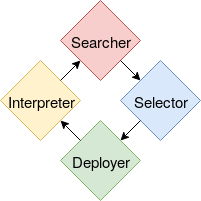
\includegraphics[scale=0.8]{Design}
\end{figure}
\section{Implementation}
\textbf{How the implementation was done and tested, with
particular focus on important / novel algorithms and/or
data structures, unusual implementation decisions, novel
user interface features, etc.}
\subsection{Searcher}
For the sake of generalizability, the available implementation of spearmint was found to be outdated and incompatible with the latest versions of various python modules planned to be used in later steps. 
Because of this, spearmint was first updated to be compatible with Python 3 and newer versions of its dependencies such as Google Protocol Buffers. This implementation of spearmint has been made available.\footnote{https://github.com/briggsby/spearmint3}
Any searcher 
\subsubsection{Bayesian Optimization - Spearmint}
% Variable for CPU can actually be an integer, which is done to the power of 2.
\subsubsection{Gradient Descent}
\subsubsection{Exhaustive search}
\subsection{Driver function}

\subsection{Selector}
% Why we only evaluated exact match. Problems with closest match. If there are architectural problems the user may want to avoid certain instance types. A selector that uses an API to retreive available instance models may be useful.
\subsubsection{Exact Match}
\subsubsection{Closest Match}
% This would require a record to be kept of previously tested instances so as not to repeat similar instances multiple times. In cases of significant noise it may be beneficial to test multiple times, so can limit this to 3.
% Driver function reads the files to make a configuration dictionary to be passed to other functons. It reads the variables into this and well as loads the functions specified in the variable file. At the end of each job, this configuration dictionary is saved as a json file for later analysis, as well as being appended to a json file that incorporates all the logs from any previous jobs performed by the function. (This file should be regularly backed up, probably into separate smaller files, as otherwise an error can throw away lots of data)
\subsection{Deployer}
\subsubsection{VM Provisioner}
\subsubsection{Docker Deployer}
\paragraph{vBench}
\paragraph{Cloudsuite3}
\paragraph{Sysbench}
\subsubsection{Ping server}

%Also fake deploy for debugging, or old_deploy for using already gathered results

\subsection{Interpreter}
% Interpreters were made for all those listed above (vBench, cloudsuite3 media streaming, sysbench
% We used very simple metrics of dividing scores (which were various measures of number of users/rate of transcoding/rate of response/number of operations) by the hourly price. This is not likely to correspond to a real metric used in business, where even a small advantage over a competitor can lead to a dramatic uptake in users, but was effective for evaluation.

\section{Evaluation}
\textbf{You should evaluate your own work with respect to your original objectives. You should also critically evaluate your work with respect to related work done by others. You should compare and contrast the project to similar work in the public domain, for example as written about in published papers, or as distributed in software available to you.}


% We were able to successfully run multiple evaluations until convergence using the system, as well as easily running exhaustive searches to then evaluate their success. We could easily replicate both cherrypick's findings, (without the log transformation) and extend to claim that multiple concurrent jobs requires a more extensive search. We showed that this works with multiple providers as well as only a single provider. We then, without using an exhaustive search, performed the experiment with the ping testing, which due to its nature was much more intensive to do exhaustive search for, which appeared to have multiple optimal options, which unsuprisingly made the Bayesian optimization much more effective.
\subsection{Configuration selection}
%cloudsuite3 media streaming was found to be extremely variable and unrelated to any hardware specs, so vBench was used for video transcoding. 
% For vBench we decided to run BO, as well as exhaustive search to them compare those findings.
\subsection{Search space selection}
% Chose cheaper options to reduce costs, and also because more powerful machines require quotas to be individually requested from the providers. Went with exact match, and as wanted to use both Amazon and Google had to categorize options. Decided to not use memory, but rather have machine type and number of CPUs, using only the first 3 machines. Further search space was unnecessary as tests always converged on the weakest machines regardless. For other perhaps more real situations, this search space could be dramatically extended, but using CPU as an integer between 1 and 6 rather than categorical, and simply having the number be to the power of 2, as these are all viable CPU options (with some slight fudging for ec2 c machines, and though it skips options of 48 and 96).


\begin{figure}
  \caption{Distribution of vBench scores}
  \centering
   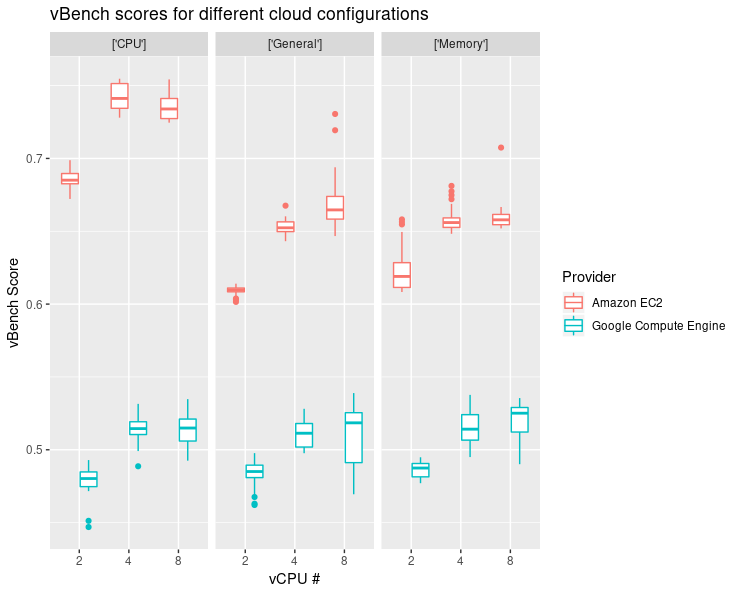
\includegraphics[scale=0.8]{vbench_scores}
\end{figure}
\begin{figure}
  \caption{Distribution of objective function values}
  \centering
   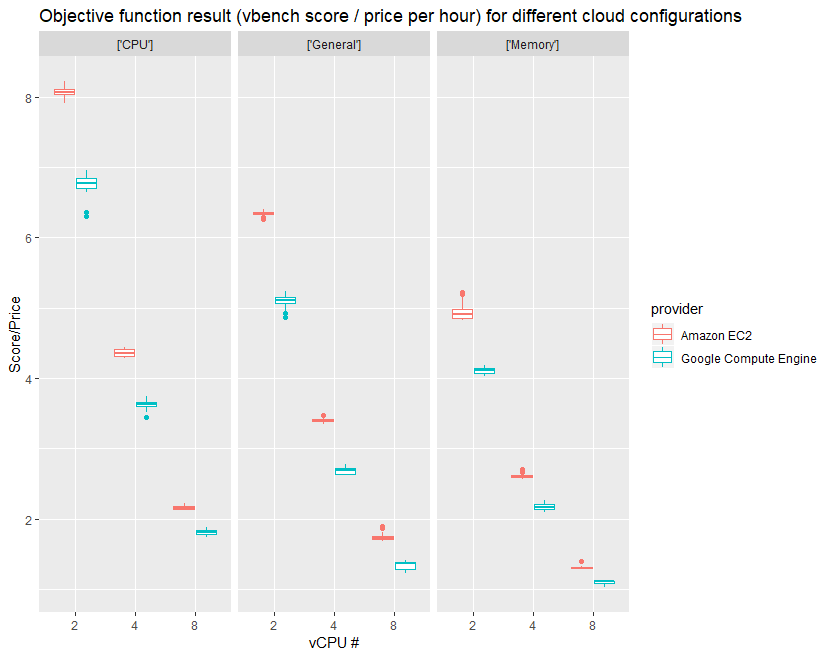
\includegraphics[scale=0.8]{vbench_values}
\end{figure}

% With the best option clearly being c5.large, running spearmint with both multiple concurrent jobs (3 simultaneous jobs)and multiple providers (both AWS and GCP), the optimal instance was selection 55\% of the time, with m5.large chosen 35\% of time. Reducing the search space significantly by reducing the number of providers to only one (GCP) causes the optimal instance to be selected instead 75\% of the time. This makes clear that for this experiment a less relaxed stopping condition may be beneficial. To attain the effectiveness that the CherryPick paper claims, we must not allow concurrent jobs. Preventing multiple jobs running at once instead ensures the optimal instance type is selected 80\% of the time. 

\subsection{Ping Test}
In the ping test evaluation of 10 spearmint experiments using the same stopping condition as above, one of two optimal configurations (AWS m5.large or c5.large instance types), with overlapping distributions for the objective value, was successfully chosen in all runs.

\section{Critical discussion}
\textbf{You should evaluate your own work with respect to your
original objectives. You should also critically evaluate
your work with respect to related work done by others.
You should compare and contrast the project to similar
work in the public domain, for example as written about
in published papers, or as distributed in software available to you. }

As mentioned, the evaluation above likely does not correspond to comparisons with which to base real deployment decisions on. In reality, a small increase in transcoding speed may lead to a far greater increase in customer uptake, rather than the effectively 1:1 ratio between price and transcoding speed assumed in the experiment. However, the evaluation shows that the methodology works very well with a given objective score measure, and it would be trivial for a new objective function to be implemented with a different relationship between the score, price, and 'value' of a given configuration.
\subsection{Future extensions}
% There is a really good space to try this with serverless computing, but cloud run is currently not supported with terraform making this more difficult.
% If time allows could write a quick bash script to try this.
% When limited to google the search space becomes much better suited for Bayesian Optimization because of the non-categorical choices with vCPU and Memory amounts
\section{Conclusions}
\textbf{You should summarise your project, emphasising your
key achievements and significant drawbacks to your
work, and discuss future directions your work could be
taken in.}
\newpage
\cite{Agarwal2012} % Just here to stop errors, delete once other citations included
\bibliographystyle{ieeetr}
\bibliography{Dissertation}
\newpage
\section*{Appendices}
\subsection*{Testing Summary}
\subsection*{User Manual}
\end{document}